\documentclass[12pt,a4paper]{article}
\usepackage[utf8]{inputenc}
\usepackage[T1]{fontenc}
\usepackage{amsmath,amsfonts,amssymb}
\usepackage{graphicx}
\usepackage{tikz}
\usetikzlibrary{shapes,arrows,positioning,trees,calc}
\usepackage{listings}
\usepackage{xcolor}

% Define custom colors
\definecolor{lightgreen}{RGB}{144,238,144}
\definecolor{lightblue}{RGB}{173,216,230}
\usepackage{geometry}
\usepackage{fancyhdr}
\usepackage{tocloft}
\usepackage{hyperref}
\usepackage{float}

\geometry{margin=1in}
\pagestyle{fancy}
\fancyhf{}
\fancyhead[L]{B-Tree Implementation Analysis}
\fancyhead[R]{\thepage}

% Code listing style
\lstset{
    language=C,
    basicstyle=\ttfamily\small,
    keywordstyle=\color{blue},
    commentstyle=\color{green!60!black},
    stringstyle=\color{red},
    numbers=left,
    numberstyle=\tiny,
    frame=single,
    breaklines=true,
    showstringspaces=false
}

% TikZ styles
\tikzset{
    btreenode/.style={
        rectangle,
        draw,
        minimum width=2cm,
        minimum height=0.8cm,
        text centered
    },
    leafnode/.style={
        btreenode,
        fill=lightblue!30
    },
    internalnode/.style={
        btreenode,
        fill=lightgreen!30
    },
    sibling/.style={
        <->,
        red,
        thick,
        bend left=30
    }
}

\begin{document}

% Title Page
\begin{titlepage}
    \centering
    \vspace*{2cm}
    
    {\Huge\textbf{B-Tree Data Structure}}\\
    \vspace{1cm}
    {\Large Implementation Analysis and Algorithm Documentation}\\
    \vspace{2cm}
    
    % B-Tree diagram on title page
    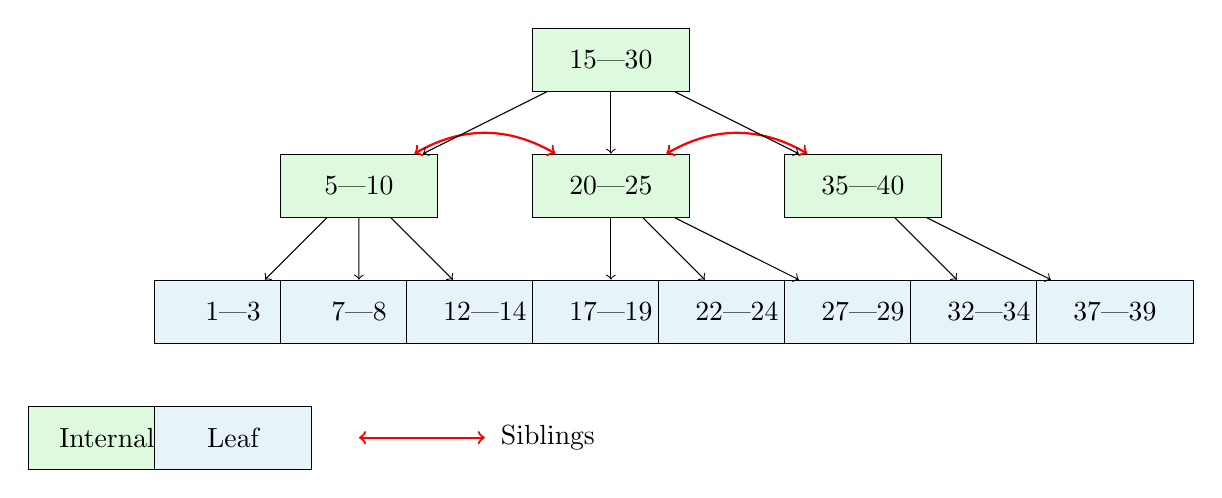
\begin{tikzpicture}[scale=0.8]
        % Root node (internal)
        \node[internalnode] (root) at (0,0) {15|30};
        
        % Level 1 internal nodes
        \node[internalnode] (left) at (-4,-2) {5|10};
        \node[internalnode] (middle) at (0,-2) {20|25};
        \node[internalnode] (right) at (4,-2) {35|40};
        
        % Sibling connections for internal nodes
        \draw[sibling] (left) to (middle);
        \draw[sibling] (middle) to (right);
        
        % Level 2 leaf nodes
        \node[leafnode] (l1) at (-6,-4) {1|3};
        \node[leafnode] (l2) at (-4,-4) {7|8};
        \node[leafnode] (l3) at (-2,-4) {12|14};
        \node[leafnode] (l4) at (0,-4) {17|19};
        \node[leafnode] (l5) at (2,-4) {22|24};
        \node[leafnode] (l6) at (4,-4) {27|29};
        \node[leafnode] (l7) at (6,-4) {32|34};
        \node[leafnode] (l8) at (8,-4) {37|39};
        
        % Parent-child connections
        \draw[->] (root) -- (left);
        \draw[->] (root) -- (middle);
        \draw[->] (root) -- (right);
        
        \draw[->] (left) -- (l1);
        \draw[->] (left) -- (l2);
        \draw[->] (left) -- (l3);
        
        \draw[->] (middle) -- (l4);
        \draw[->] (middle) -- (l5);
        \draw[->] (middle) -- (l6);
        
        \draw[->] (right) -- (l7);
        \draw[->] (right) -- (l8);
        
        % Legend
        \node[internalnode] at (-8,-6) {Internal};
        \node[leafnode] at (-6,-6) {Leaf};
        \draw[sibling] (-4,-6) -- (-2,-6);
        \node at (-1,-6) {Siblings};
    \end{tikzpicture}
    
    \vspace{2cm}
    {\Large Database Systems Implementation}\\
    \vspace{0.5cm}
    {\normalsize Analysis of Disk-Based C Implementation}\\
    \vspace{2cm}
    {\large \today}
    
\end{titlepage}

\tableofcontents
\newpage

\section{Introduction}

B-Trees are self-balancing tree data structures that maintain sorted data and allow searches, sequential access, insertions, and deletions in logarithmic time. This document analyzes a specific C implementation of a B-Tree designed for database storage systems with disk-based persistence.

The implementation features several key characteristics:
\begin{itemize}
    \item Disk-based storage with block-level I/O operations
    \item Sibling relationships maintained only for internal nodes
    \item Dynamic node splitting and merging operations
    \item Support for both search and modification operations
\end{itemize}

\section{Data Structure Overview}

\subsection{BTreeNode Structure}

The core data structure is the \texttt{BTreeNode}, which represents both internal and leaf nodes:

\begin{lstlisting}
typedef struct BTreeNode {
    uint64_t block_number;      // Physical block number on disk
    bool is_leaf;              // Whether this is a leaf node
    uint64_t key;              // Actual key (for leaf nodes)
    uint64_t value;            // Associated value for key-value pairs
    uint16_t num_keys;         // Current number of keys in node
    uint64_t keys[MAX_KEYS];   // Array of keys
    uint64_t children[MAX_KEYS + 1]; // Child block numbers (internal only)
    uint64_t parent;           // Parent node block number (0 if root)
    uint64_t left_sibling;     // Left sibling (internal nodes only)
    uint64_t right_sibling;    // Right sibling (internal nodes only)
} BTreeNode;
\end{lstlisting}

\subsection{Sibling Relationship Management}

A critical aspect of this implementation is that \textbf{only internal nodes maintain sibling relationships}. The \texttt{left\_sibling} and \texttt{right\_sibling} fields are:

\begin{itemize}
    \item Set to meaningful values only for internal nodes
    \item Set to 0 for leaf nodes and the root node
    \item Updated during split and merge operations
    \item Used for efficient traversal and rebalancing
\end{itemize}

\begin{figure}[H]
\centering
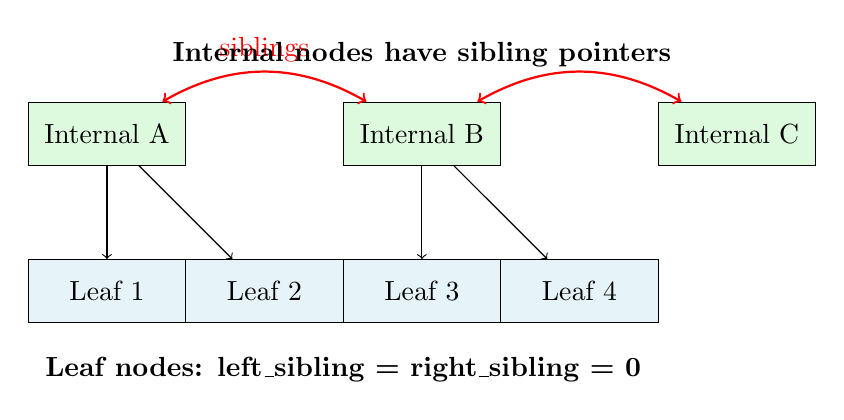
\begin{tikzpicture}
    % Internal nodes with siblings
    \node[internalnode] (int1) at (0,2) {Internal A};
    \node[internalnode] (int2) at (4,2) {Internal B};
    \node[internalnode] (int3) at (8,2) {Internal C};
    
    % Sibling connections
    \draw[sibling] (int1) to node[above] {siblings} (int2);
    \draw[sibling] (int2) to (int3);
    
    % Leaf nodes (no siblings)
    \node[leafnode] (leaf1) at (0,0) {Leaf 1};
    \node[leafnode] (leaf2) at (2,0) {Leaf 2};
    \node[leafnode] (leaf3) at (4,0) {Leaf 3};
    \node[leafnode] (leaf4) at (6,0) {Leaf 4};
    
    % Parent-child connections
    \draw[->] (int1) -- (leaf1);
    \draw[->] (int1) -- (leaf2);
    \draw[->] (int2) -- (leaf3);
    \draw[->] (int2) -- (leaf4);
    
    % Annotations
    \node at (4,3) {\textbf{Internal nodes have sibling pointers}};
    \node at (3,-1) {\textbf{Leaf nodes: left\_sibling = right\_sibling = 0}};
\end{tikzpicture}
\caption{Sibling Relationship Structure}
\end{figure}

\section{Core Algorithms}

\subsection{Search Algorithm}

The search operation traverses the tree from root to leaf, following the appropriate child pointers based on key comparisons.

\begin{figure}[H]
\centering
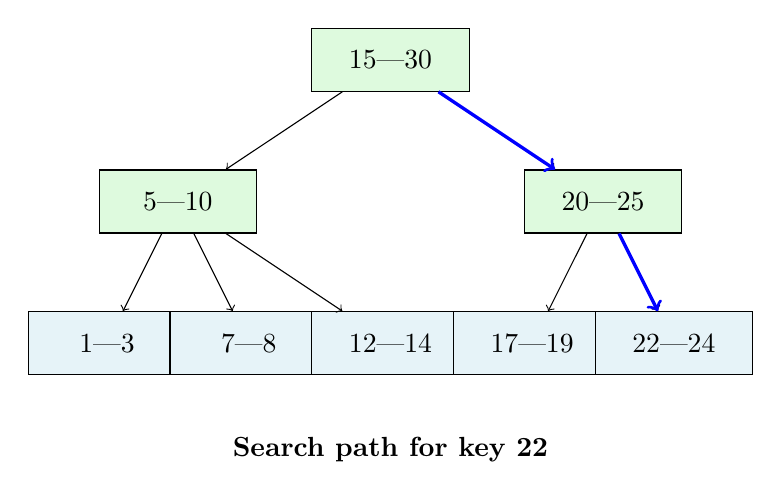
\begin{tikzpicture}[scale=0.9]
    % Tree structure
    \node[internalnode] (root) at (0,0) {15|30};
    \node[internalnode] (left) at (-3,-2) {5|10};
    \node[internalnode] (right) at (3,-2) {20|25};
    \node[leafnode] (ll) at (-4,-4) {1|3};
    \node[leafnode] (lm) at (-2,-4) {7|8};
    \node[leafnode] (lr) at (0,-4) {12|14};
    \node[leafnode] (rl) at (2,-4) {17|19};
    \node[leafnode] (rm) at (4,-4) {22|24};
    
    % Connections
    \draw[->] (root) -- (left);
    \draw[->] (root) -- (right);
    \draw[->] (left) -- (ll);
    \draw[->] (left) -- (lm);
    \draw[->] (left) -- (lr);
    \draw[->] (right) -- (rl);
    \draw[->] (right) -- (rm);
    
    % Search path for key 22
    \draw[->, very thick, blue] (root) -- (right);
    \draw[->, very thick, blue] (right) -- (rm);
    
    \node at (0,-5.5) {\textbf{Search path for key 22}};
\end{tikzpicture}
\caption{B-Tree Search Operation}
\end{figure}

\textbf{Algorithm Steps:}
\begin{enumerate}
    \item Start at root node
    \item Compare search key with node keys
    \item If leaf node: return success/failure
    \item If internal node: follow appropriate child pointer
    \item Repeat until key found or leaf reached
\end{enumerate}

\subsection{Insertion Algorithm}

Insertion maintains the B-Tree properties through node splitting when nodes become full.

\begin{figure}[H]
\centering
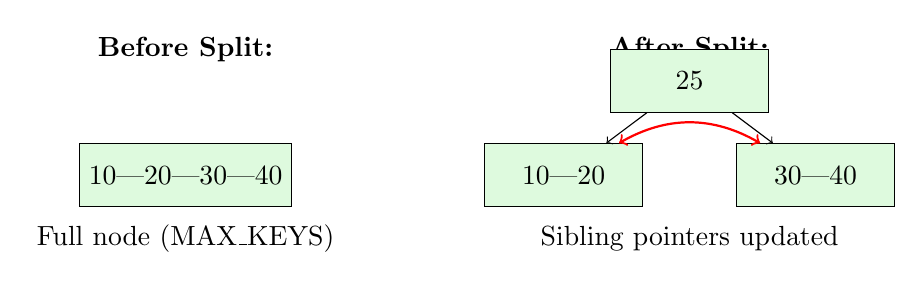
\begin{tikzpicture}[scale=0.8]
    % Before split
    \node at (-6,2) {\textbf{Before Split:}};
    \node[internalnode] (before) at (-6,0) {10|20|30|40};
    \node at (-6,-1) {Full node (MAX\_KEYS)};
    
    % After split
    \node at (2,2) {\textbf{After Split:}};
    \node[internalnode] (left_after) at (0,0) {10|20};
    \node[internalnode] (right_after) at (4,0) {30|40};
    \draw[sibling] (left_after) to (right_after);
    
    \node[internalnode] (parent) at (2,1.5) {25};
    \draw[->] (parent) -- (left_after);
    \draw[->] (parent) -- (right_after);
    
    \node at (2,-1) {Sibling pointers updated};
\end{tikzpicture}
\caption{Node Splitting During Insertion}
\end{figure}

\textbf{Key Points:}
\begin{itemize}
    \item When a node splits, sibling pointers are established between the two new internal nodes
    \item The median key is promoted to the parent
    \item Leaf nodes do not maintain sibling relationships
    \item Root splitting creates a new root level
\end{itemize}

\subsection{Deletion Algorithm}

Deletion is more complex, involving borrowing from siblings or merging nodes when they become too sparse.

\begin{figure}[H]
\centering
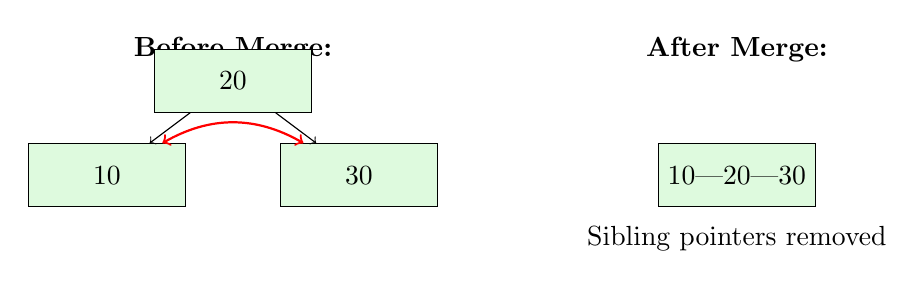
\begin{tikzpicture}[scale=0.8]
    % Before merge
    \node at (-6,2) {\textbf{Before Merge:}};
    \node[internalnode] (left_before) at (-8,0) {10};
    \node[internalnode] (right_before) at (-4,0) {30};
    \draw[sibling] (left_before) to (right_before);
    \node[internalnode] (parent_before) at (-6,1.5) {20};
    \draw[->] (parent_before) -- (left_before);
    \draw[->] (parent_before) -- (right_before);
    
    % After merge
    \node at (2,2) {\textbf{After Merge:}};
    \node[internalnode] (merged) at (2,0) {10|20|30};
    \node at (2,-1) {Sibling pointers removed};
\end{tikzpicture}
\caption{Node Merging During Deletion}
\end{figure}

\textbf{Merge Process:}
\begin{enumerate}
    \item Identify underflowing nodes
    \item Attempt to borrow from siblings (if they have extra keys)
    \item If borrowing fails, merge with a sibling
    \item Update sibling pointers after merge
    \item Recursively handle parent node changes
\end{enumerate}

\section{Disk Interface Integration}

The B-Tree implementation integrates with a disk interface for persistent storage:

\begin{lstlisting}
typedef struct DiskInterface {
    int disk_file;                   // File handle
    void* disk_base;                 // Memory-mapped base
    uint64_t total_blocks;           // Total blocks available
    bool is_mounted;                 // Mount status
} DiskInterface;
\end{lstlisting}

\textbf{Key Operations:}
\begin{itemize}
    \item \texttt{disk\_read\_block()}: Load node from disk
    \item \texttt{disk\_write\_block()}: Persist node to disk
    \item \texttt{alloc\_page()}: Allocate new disk block
    \item \texttt{free\_page()}: Deallocate disk block
\end{itemize}

\section{Implementation Functions}

\subsection{Node Management}
\begin{itemize}
    \item \texttt{btree\_node\_create()}: Allocate and initialize new node
    \item \texttt{btree\_node\_free()}: Deallocate node and free disk block
    \item \texttt{btree\_node\_read()}: Load node from disk block
    \item \texttt{btree\_node\_write()}: Save node to disk block
\end{itemize}

\subsection{Tree Operations}
\begin{itemize}
    \item \texttt{btree\_search()}: Find key in tree
    \item \texttt{btree\_insert()}: Add new key-value pair
    \item \texttt{btree\_delete()}: Remove key from tree
    \item \texttt{btree\_print()}: Display tree structure
\end{itemize}

\subsection{Structural Operations}
\begin{itemize}
    \item \texttt{btree\_split\_child()}: Split full child node
    \item \texttt{btree\_merge\_children()}: Merge sparse sibling nodes
    \item \texttt{btree\_update\_parent\_keys()}: Maintain parent key consistency
    \item \texttt{btree\_borrow\_left/right()}: Redistribute keys between siblings
\end{itemize}

\section{Sibling Management Details}

\subsection{Split Operation Sibling Updates}

When an internal node splits:
\begin{enumerate}
    \item Create two new nodes from the original
    \item Set \texttt{left\_sibling} and \texttt{right\_sibling} between the new nodes
    \item Update any existing sibling relationships
    \item Leaf nodes created during splits maintain \texttt{left\_sibling = right\_sibling = 0}
\end{enumerate}

\subsection{Merge Operation Sibling Updates}

When internal nodes merge:
\begin{enumerate}
    \item Combine keys from both nodes
    \item Update sibling pointers to skip the merged node
    \item Set merged node's sibling pointers to 0
    \item Free the now-unused node
\end{enumerate}

\section{Performance Characteristics}

\begin{itemize}
    \item \textbf{Search}: O(log n) time complexity
    \item \textbf{Insert}: O(log n) amortized time
    \item \textbf{Delete}: O(log n) amortized time
    \item \textbf{Space}: O(n) space complexity
    \item \textbf{Disk I/O}: Minimized through block-based operations
\end{itemize}

\section{Conclusion}

This B-Tree implementation provides an efficient, disk-based data structure suitable for database systems. The key design decisions include:

\begin{itemize}
    \item Sibling relationships maintained only for internal nodes
    \item Disk-based persistence with block-level I/O
    \item Standard B-Tree balancing through splits and merges
    \item Support for both point queries and range operations
\end{itemize}

The restriction of sibling pointers to internal nodes simplifies the implementation while maintaining the essential properties needed for efficient tree traversal and rebalancing operations.

\end{document}
